\section{Results}

\subsection{Online clustering}

\subsubsection{Setup}

The online clustering is done on a simulated stream of news articles based on the same data set as used in the clustering evaluation. This allows for direct comparison between the detected events and the ground truth. The settings to run the clustering are as follows:

\begin{itemize}
    \item Preprocessing: Text lemmatisation
    \item Vector space model: tf-idf
    \item Clustering method: HDBSCAN
    \item Minimum cluster size: 6
    \item Distance metric: cosine
\end{itemize}

The clustering is run over 30 days with a total of 42'916 news articles. The distribution of news articles this time period is illustrated in Figure \ref{fig:news_articles_over_time}. The time delta, which is the amount of time between two batches, is set to one hour. 

\begin{figure}[h]
    \centering
    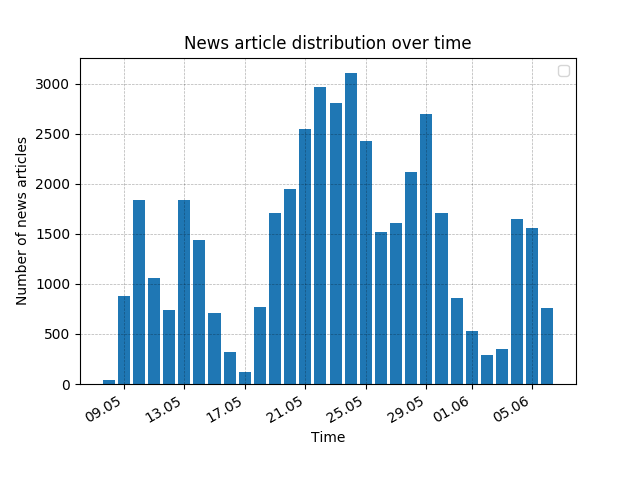
\includegraphics[width=0.5\textwidth]{news_articles_over_time}
    \caption{Incoming news articles over 30 days}
    \label{fig:news_articles_over_time}
\end{figure}

\subsubsection{Evaluation}

The goal of the online clustering is to detect new events in an incoming stream of news articles and changes in existing events. This evaluation analyses the results of our simulated test runs with different batch sizes.

We start the evaluation with using a fixed batch size. Figure \ref{fig:event_detection_differences} shows the differences between the number of detected events and the number of true events for both new and existing topics. Based on this data we see the impact of different batch sizes for the accuracy in detected events. The difference with a batch size of 5000 news articles is fairly lower than the batch size of 1000. The difference is especially noticeable in the time period between the 21.05 and 25.05. The reason for this spike can be found in the distribution of incoming news articles as shown in Figure \ref{fig:news_articles_over_time}. During this period we receive up to 3000 news articles in a single day. This means by using a lower batch size such as 1000, the overlap between batches gets too small to reliably detect changes between batches, which causes too many new topics to be detected. 

\begin{figure}[h]
    \centering
    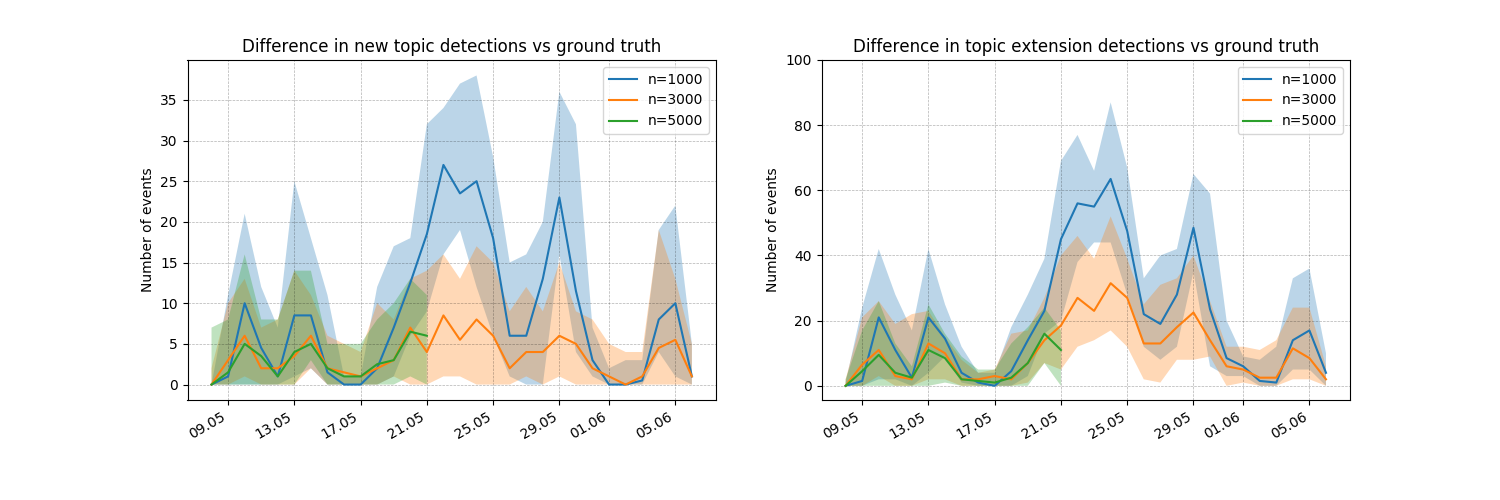
\includegraphics[width=1\textwidth]{event_detection_differences}
    \caption{Comparison between the difference in detected and true events. The line represents the median, while the area shows the range from the minimum to the maximum value}
    \label{fig:event_detection_differences}
\end{figure}

Although a larger batch size does not simply equal a better difference, as can be seen in Figure \ref{fig:event_detection_differences} by comparing the differences using a batch size of 3000 with a batch size of 5000. The batch size n=3000 shows a generally lower difference in the detection of new events than with n=5000. The differences between both batch sizes are less significant when detecting changes in existing events.

Based on the overall differences, we do not know the accuracy of those predictions. 
If the difference between newly detected events and true events is zero, there is still the possibility, that the events itself are different from the ground truth, and thus contain false positives. To measure the quality of events, we can look at the collection of events in a single batch as a subset of clusters, where each event is represented by a cluster containing all relevant news articles. Since we now have two clusterings, one containing detected events and the other with events taken from the ground truth, we can apply our MP-Score as a metric to get an insight into the quality of the detected events over the ground truth. Figure \ref{fig:event_detection_mp_score_1000} shows the MP-Scores for an online clustering using a batch size of 1000. Since there is quite a large variance, the score is shown as a boxplot, where a single box represents a full day. The large variance is already the first indication, that the quality is rather low. Meaning that there are still many false positives and false negatives.

\begin{figure}[h]
    \centering
    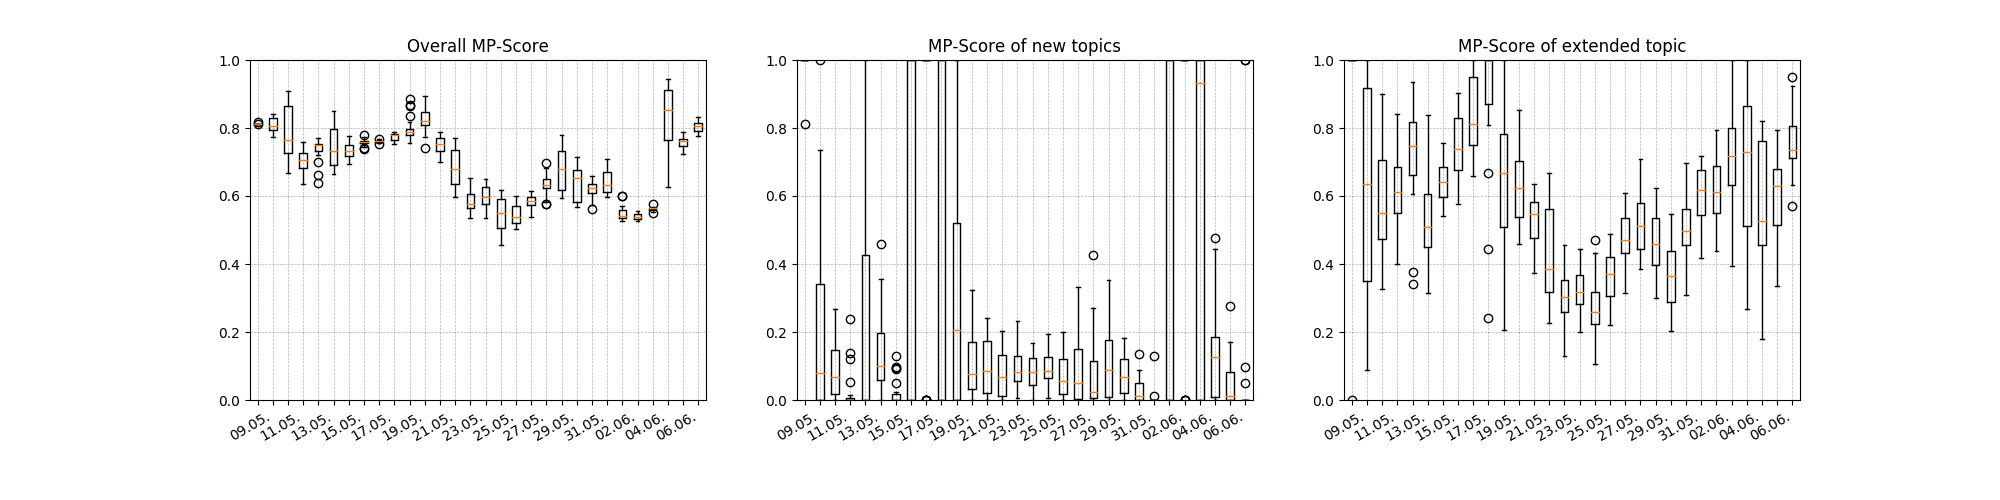
\includegraphics[width=1\textwidth]{event_detection_mp_score_1000}
    \caption{MP-Scores for clusterings using batch size of 1000}
    \label{fig:event_detection_mp_score_1000}
\end{figure}

Looking at an increased batch size of 5000 in Figure \ref{fig:event_detection_mp_score_5000}, we note that there is less variance in the overall MP-Score, which compares the full clustering with the ground truth. Although the variance for new and existing event detections is still fairly high. Additionally while the variance is high, the median for new topics is mostly around 0.1. This tells us that most of the newly detected events do not correspond with new events according to the ground truth. The detection of extensions of existing events is generally more accurate with a median between 0.5 and 0.8 using n=5000, but there is still are wide variance noticeable.

\begin{figure}[h]
    \centering
    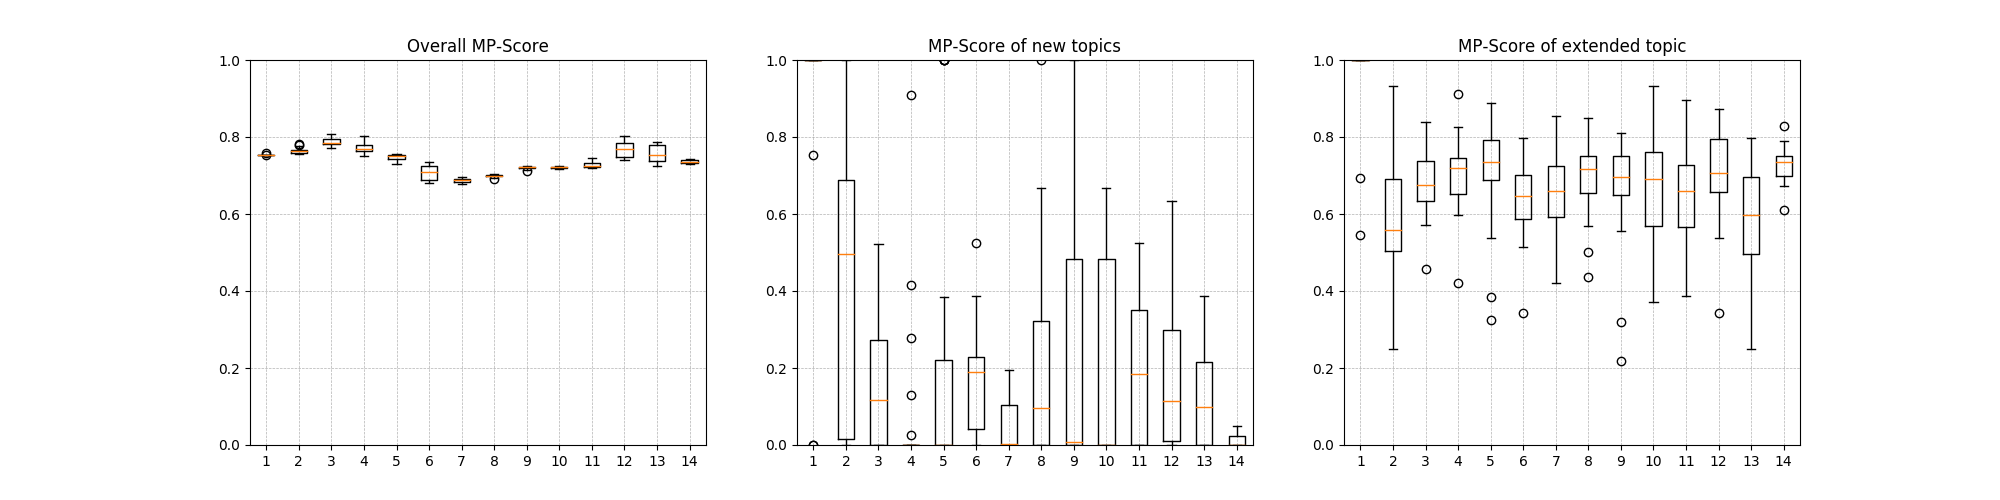
\includegraphics[width=1\textwidth]{event_detection_mp_score_5000}
    \caption{MP-Scores for clusterings using batch size of 5000}
    \label{fig:event_detection_mp_score_5000}
\end{figure}

One of the reasons for the difference in the accuracy of the detection of new events and the extension of events might be explained by the $min\_cluster\_size$. In the current setting the $min\_cluster\_size$ is set to 5, which means if an event occurs in batch one containing only four news articles, it will be discarded as noise. If the second batch contains additional news articles for the same event, it will be detected as a new occurrences, but the ground truth treats it as an existing event. To see how this affects the result we run the same simulation with a batch size of n=3000 a second time, but only considering new events from the ground truth if the number of news articles is greater or equal to the $min\_cluster\_size$.

\begin{figure}[h]
    \centering
    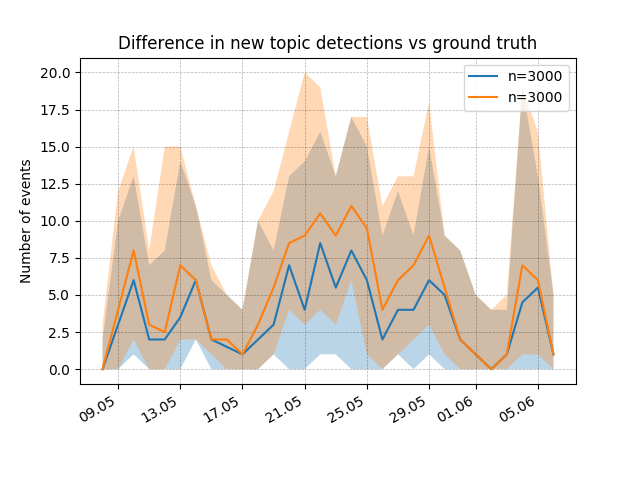
\includegraphics[width=0.5\textwidth]{event_detection_differences_with_min_cluster_size}
    \caption{Differences in predictions vs ground truth using batch size of 3000.}
    \label{fig:event_detection_differences_with_min_cluster_size}
\end{figure}

Limiting new events in the ground truth based on the $min\_cluster\_size$ gives the opposite result as initially expected. 
Figure \ref{fig:event_detection_differences_with_min_cluster_size} clearly shows an increase in the difference between predicted events and the adjusted ground truth. This means we already detected more new events than there were present in the ground truth and limiting it based on the $min\_cluster\_size$ only lowered the true number of events, thus leading to an increase in the difference. A look at the raw data from an initial simulation run in Figure \ref{fig:event_detection_by_date_3000} validates this assumption.

\begin{figure}[h]
    \centering
    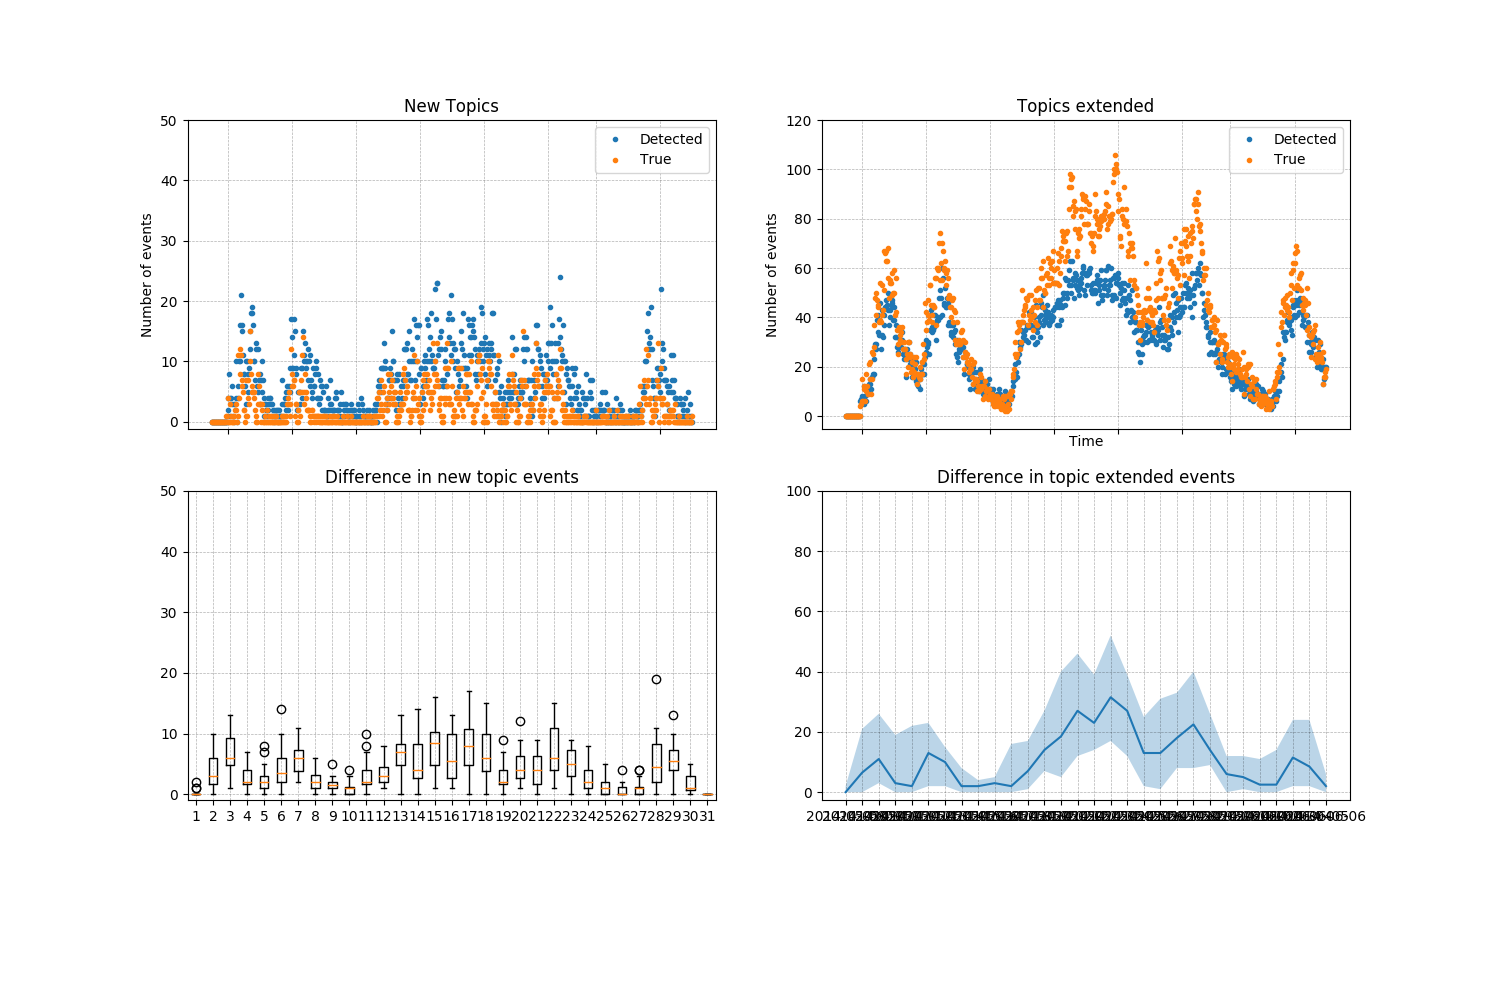
\includegraphics[width=1\textwidth]{event_detection_by_date_3000}
    \caption{Number of events with a batch size of 3000}
    \label{fig:event_detection_by_date_3000}
\end{figure}

The raw data in Figure \ref{fig:event_detection_by_date_3000} also shows a direct correlation between the number of detected new events and the number of detected changes in events. The more changes we missed, the more new events are detected. This is to be expected, since the detection of changes depends upon finding similar pairs of clusters in two different batches. If a cluster in the current batch could not be matched to a cluster from the previous batch, the cluster from the current batch will be seen as a new event. Therefore the accuracy in finding pairs of clusters in crucial to a better performance. The online clustering makes use of Locality Sensitive Hashing as explained in section \ref{sec:online_clustering_implementation}. The current threshold value for determining the similarity is set to 0.75. To see the impact on the similarity threshold, we run the online clustering again with a batch size of n=3000 and different threshold values.

\begin{figure}[h]
    \centering
    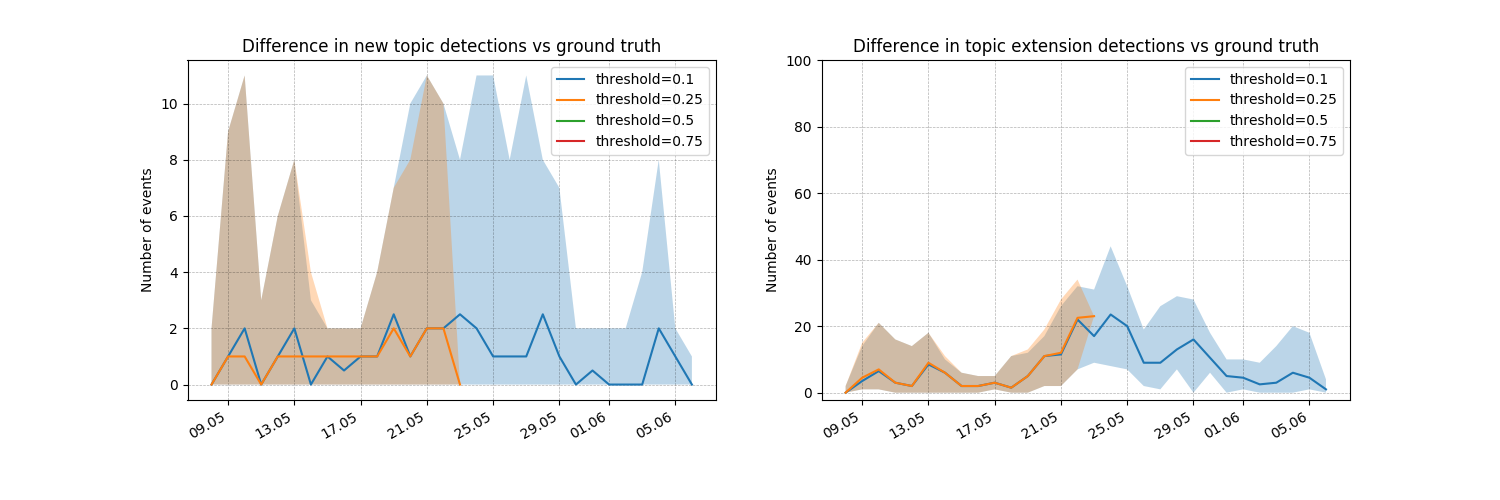
\includegraphics[width=1\textwidth]{event_detection_differences_threshold}
    \caption{Differences in detected over true events with different thresholds}
    \label{fig:event_detection_differences_threshold}
\end{figure}

Figure \ref{fig:event_detection_differences_threshold} shows the effect of the threshold on the difference in decided over true events. We see how the initial threshold of 0.75 was set too high, as lower threshold values such as 0.1 provide a significant lower difference. While there is still a substantial variance per day the median of 0.1 and 0.5 is generally more stable and lower than with a threshold value of 0.75. The reason for the better performance of lower threshold values, is that the overlap between batches decreases with an increase in the volume of news articles. This is clearly visible during the peaks in Figure \ref{fig:event_detection_differences_threshold}. Thus a high similarity threshold cannot be met, since there exists only an overlap of a few news articles for the same cluster between batches. The MP-Score is also improved for new events as can be seen in Figure \ref{fig:event_detection_mp_score_3000_0_1}. While there is more variance than in similar plots from Figure \ref{fig:event_detection_mp_score_1000} and Figure \ref{fig:event_detection_mp_score_5000}, the median from using threshold=0.1 clearly surpasses any measure from using threshold=0.75. The high variance in the boxplot is due to the fact, that there are only a few new events per hour, if any. This means detecting no events, when there are none leads to a score of 1, while detecting one event, when there is none leads to a score of 0.

\begin{figure}[h]
    \centering
    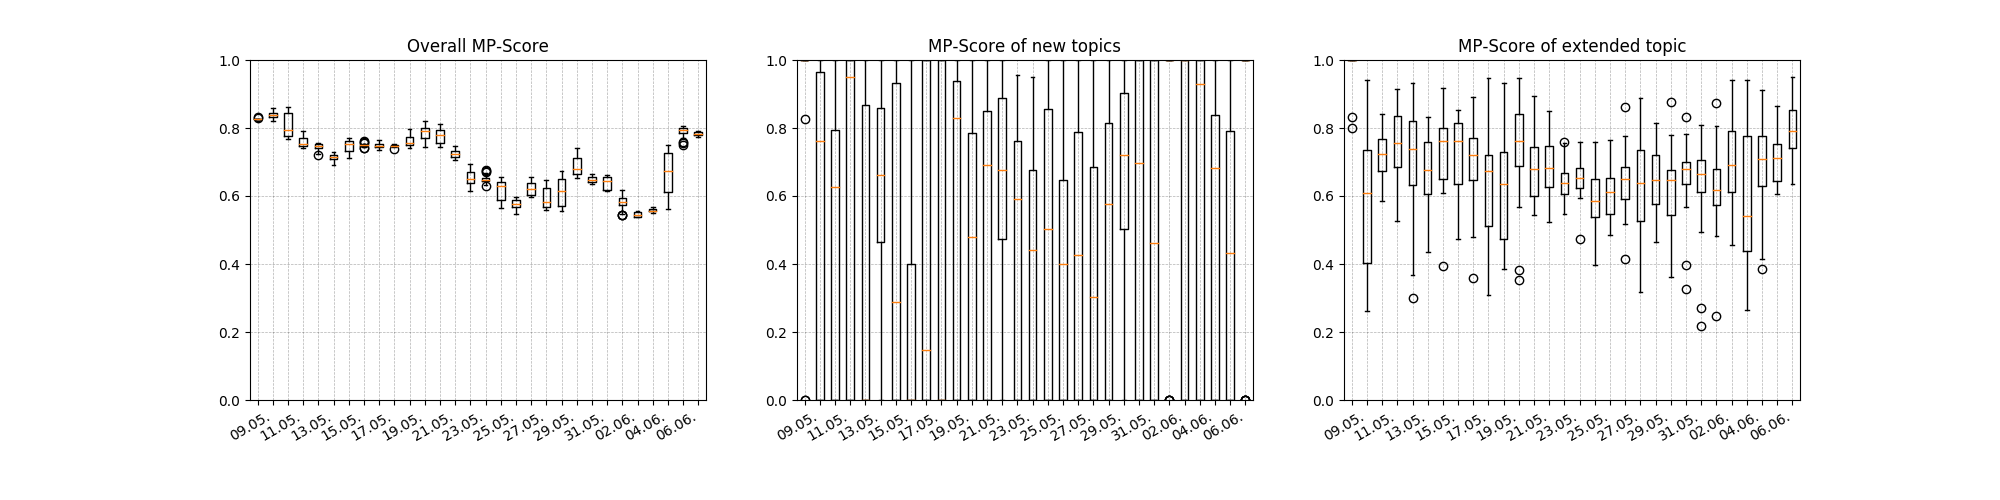
\includegraphics[width=1\textwidth]{event_detection_mp_score_3000_0_1}
    \caption{MP-Scores for online clustering with batch size n=3000 and threshold=0.1}
    \label{fig:event_detection_mp_score_3000_0_1}
\end{figure}

After having analysed the impact of different batch sizes and the similarity threshold, we want to explore the result of using a dynamic batch size. The first dynamic method loads the number of samples over $n$ hours. The second dynamic method calculates the batch size based on the incoming samples and a predefined factor. 

Figure \ref{fig:event_detection_differences_hours} shows the difference in detected events compared with the true number of events using the first dynamic method.  

\begin{figure}[h]
    \centering
    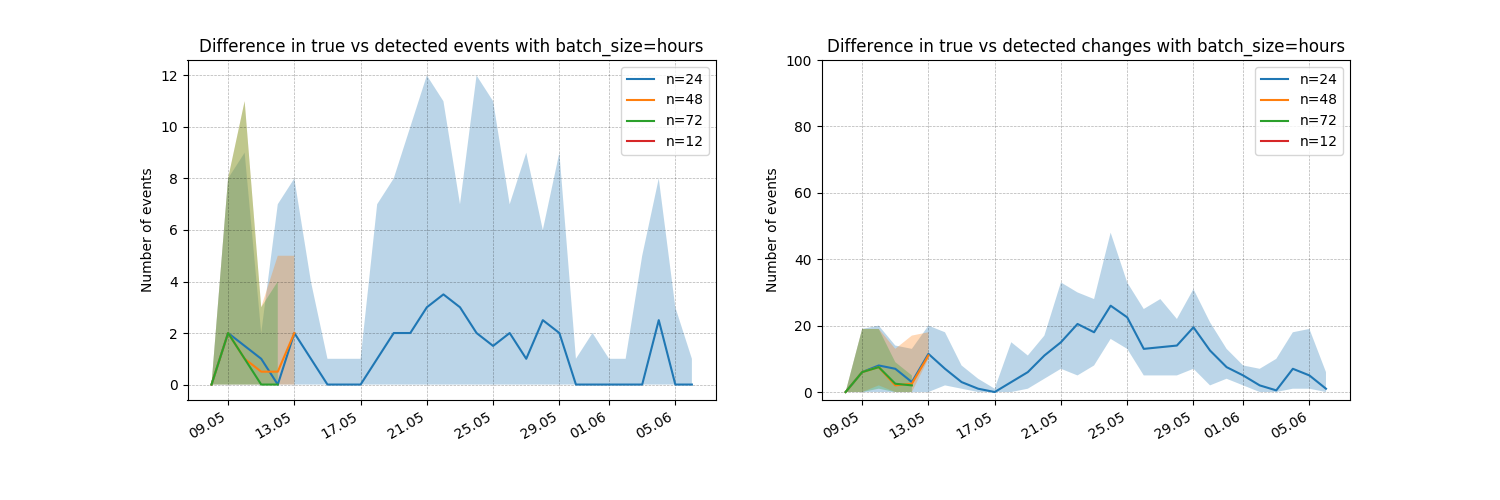
\includegraphics[width=1\textwidth]{event_detection_differences_hours}
    \caption{Difference in detected events vs predict events by using a dynamic batch size based on hours.}
    \label{fig:event_detection_differences_hours}
\end{figure}

\begin{figure}[h]
   \centering
   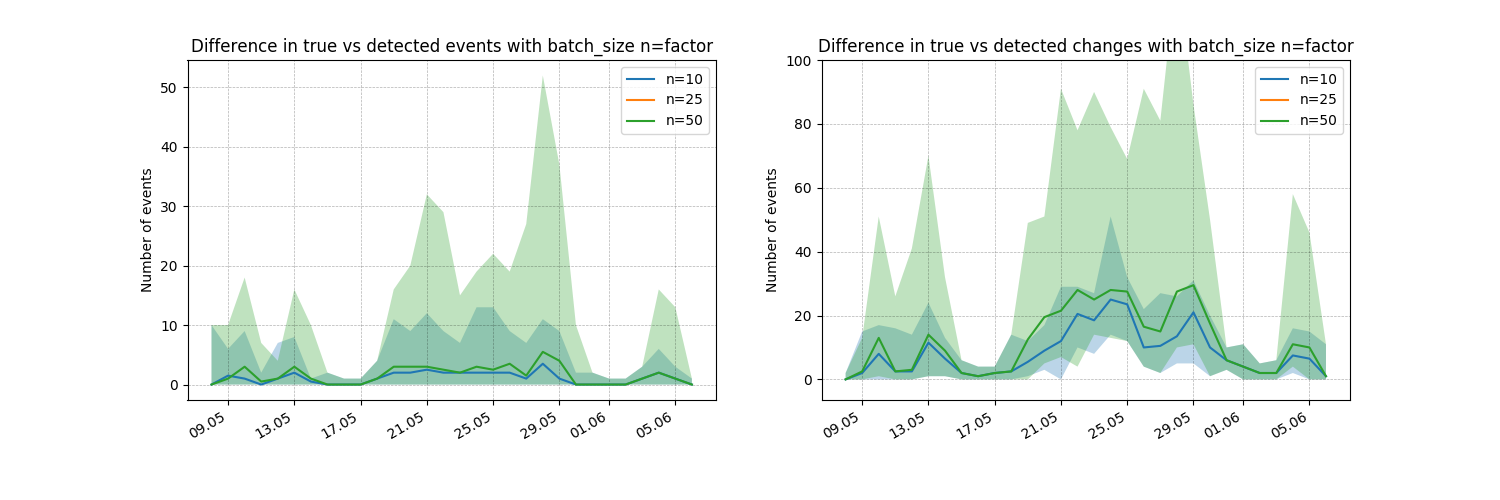
\includegraphics[width=1\textwidth]{event_detection_differences_relative}
   \caption{Difference in detected events vs predict events by using a dynamic batch size based on incoming samples.}
   \label{fig:event_detection_differences_relative}
\end{figure}



\begin{table}[h]
    \centering
    \begin{tabular}{|r|r|r|}
        \hline
        \textbf{Batch size method} & \textbf{Median} & \textbf{Standard deviation} \\
        \hline
        Fixed & 0 & 0 \\ \hline
        Time based & 0 & 0 \\ \hline
        Relative & 0 & 0 \\ \hline
    \end{tabular}
    \caption{Final scores obtained by each method for setting the batch size.}
    \label{tab:batch_size_methods}
\end{table}

%% Refactor:
Additional reasons for the general low performance in the quality of events might be due to the noise rate and the difference in the number of news articles. As described in the section about the cluster method evaluation, the noise rate for sample sizes between 1000 and 5000 ranges from 20\% to 30\%. This means a significant amount gets discarded as noise and thus potential new events might not even be detected, because too many of their news articles are discarded. Once an event is detected, detection in changes are more reliable than for new events, but as the variance in the MP-Score shows, there is still a fairly large error rate.

% TODO how large?

%% Refactor:
% As a final note let us look at two specific examples. One where the detection was mostly accurate and a second where the detection failed. Figure \ref{fig:online_clustering_example_gmail} shows the result for the story regarding the "Gmail redesign". Each dot represents one or more news articles, which appear at a certain time in the data stream. All news articles belong to the same story. As we can see after five news articles appearing in the stream, a new event is detected marked as green. Following the new event, additional news articles are clustered and detected as part of the existing event marked as blue. The last cluster does not contain all news articles any more, since the first few articles were not part of the last batch. However there is still enough overlap with the cluster from the previous batch, to match this cluster to the existing event about the "Gmail redesign". This example shows a good example of how the online clustering works in the optimal case.

% \begin{figure}[h]
%     \centering
%     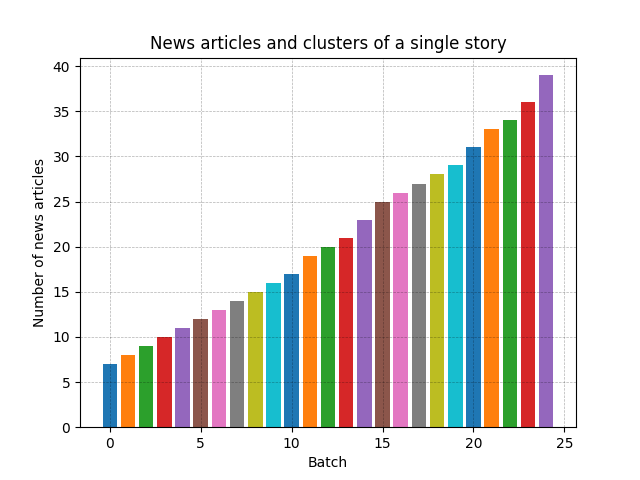
\includegraphics[width=1\textwidth]{online_clustering_example_gmail}
%     \caption{News articles belonging to the story "Gmail redesign" together with clusters, where they appear in. The circles represent incoming news articles at a specific time. The rectangles show which news articles are contained within a cluster. New clusters are marked as green and existing cluster are blue.}
%     \label{fig:online_clustering_example_gmail}
% \end{figure}

% The second example shown in Figure \ref{fig:online_clustering_example_neighbours} illustrates the opposite case, where the events do not match well with the ground truth. All news articles in this example belong to a story about the release of new film called "Bad Neighbours". Black dots indicate news articles, which do not appear in any cluster. The fragmentation of the clusters themselves clearly shows, that many of these news articles have been matched with different stories and therefore in different events. 

% \begin{figure}[h]
%     \centering
%     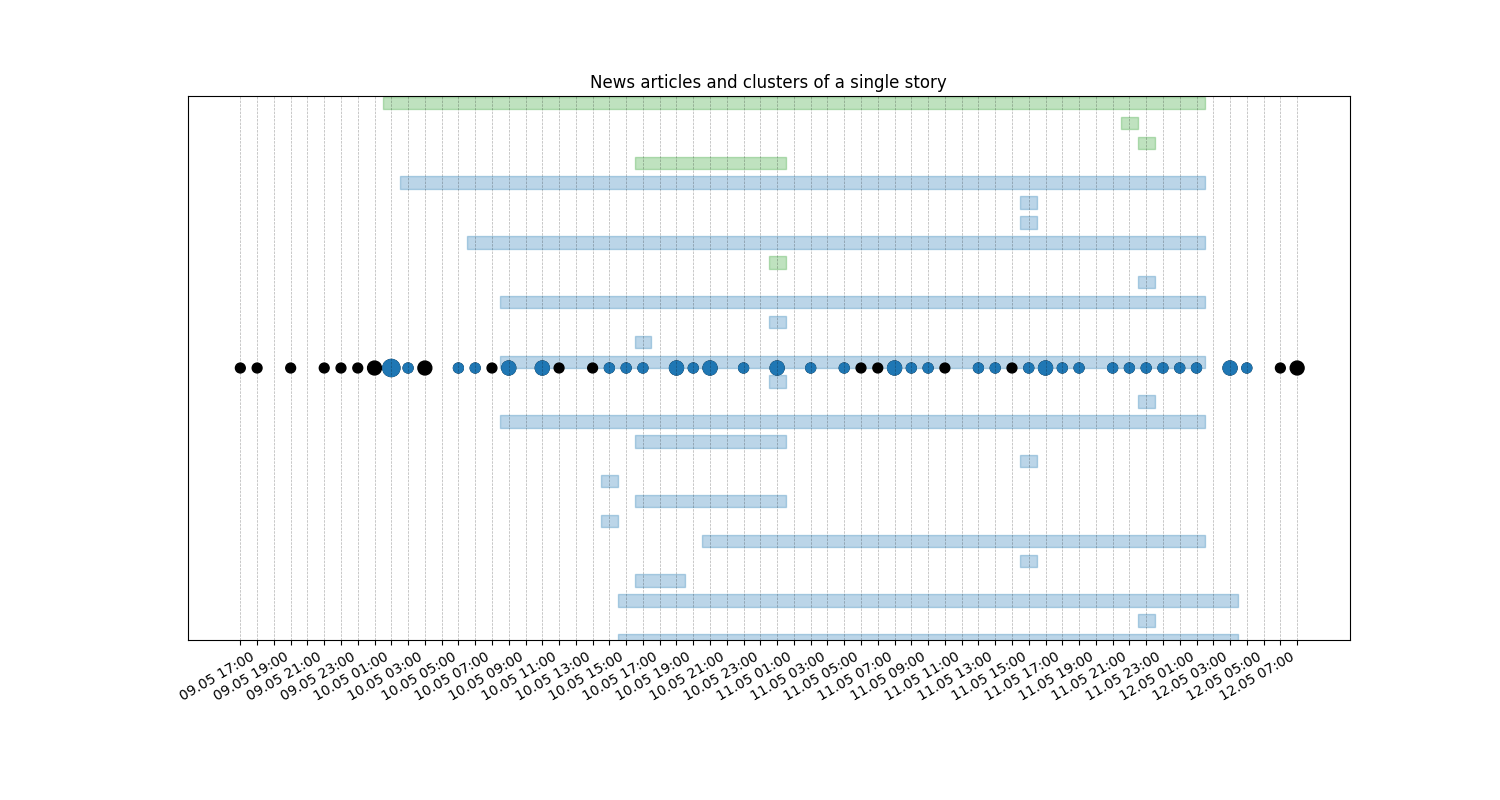
\includegraphics[width=1\textwidth]{online_clustering_example_neighbours}
%     \caption{News articles belonging to the story "Bad Neighbours" together with clusters, where they appear in. Circles marked as black represent news articles, which do not appear in any cluster.}
%     \label{fig:online_clustering_example_neighbours}
% \end{figure}

% The difference in the performance of both examples, can be explained based on the news articles themselves. The first example about the "Gmail redesign" consists mostly of press releases, technology focused news sites such as \textit{Ars Technica} or \textit{PC Magazine}. Therefore the contents of the news articles are of high quality and share the same technical vocabulary. The second example with the new release of the movie "Bad Neighbours" has a wider variety of sources and types of articles. Some news articles are short summaries, while others are interviews or personal reviews. Additionally the vocabulary is more general than compared to technical articles and varies stronger between articles. This might lead to differences in the tf-idf model, causing the articles to be not considered similar enough to belong to the same cluster, as was shown in the clustering method evaluation with Table \ref{tab:clustering_example_features}.

\subsubsection{Conclusion}

While the overall clustering results in good scores, the detection of new events and changes in existing events is more sensible to smaller inaccuracies and the volume of incoming data. We explored different settings for the batch size, threshold values and looked at two specific examples for different clusters. It turned out our initial similarity threshold value was set too high and lowering the value resulted in a significant improvement detecting new events. Although the overall performance was still very varied. Possible reasons have been explored such as the $min\_cluster\_size$, the noise rate, the general difference in the number of news articles or the vector space model representing news articles. As a result we conclude that the accuracy of the clustering method used in this approach is insufficient for the detection of events in a news stream, but it would be certainly interesting to see it be applied with different kinds of textual data streams. 